\documentclass{beamer}

% Metadata
\title{Statische Typsysteme für JavaScript}
\subtitle{Entwicklung eines Transpilers zur Übersetzung von Flow nach TypeScript}
\author{Jonathan Gruber}
\institute{HTWK Leipzig}
\date{18. Dezember 2019}

% Encoding
\usepackage[utf8]{inputenc}
\usepackage[T1]{fontenc}

% Babel
\usepackage[ngerman]{babel}

% Fonts
\usepackage{arev} % for Math
\usepackage[sb]{plex-sans}
\usepackage[scale=0.8,sb]{plex-mono}

% Biber (references)
\usepackage[backend=biber]{biblatex}
\addbibresource{src/references.bib}

\let\OLDitemize\itemize
\renewcommand\itemize{\OLDitemize\addtolength{\itemsep}{4pt}}

\let\OLDenumerate\enumerate
\renewcommand\enumerate{\OLDenumerate\addtolength{\itemsep}{2pt}}

\usepackage{csquotes}
\usepackage{longtable, tabu, booktabs}
\usepackage{tikz}
\usepackage{hyperref}

% Code listings
\usepackage{listings}

\lstset{
  aboveskip=0pt,
  basicstyle=\linespread{1.04}\small\ttfamily,
  belowcaptionskip=0pt,
  belowskip=0pt,
  breakatwhitespace=true,
  breaklines=true,
  comment=[l]{//},
  commentstyle=\color{darkgray},
  emph={?, any, Array, boolean, empty, interface, mixed, never, number, null, opaque, string, this, unknown, void, T, TypeAlias},
  emphstyle=\itshape,
  extendedchars=false,
  keywords={abstract, arguments, await, boolean, break, byte, case, catch, char, class, const, continue, debugger, declare, default, delete, do, double, else, enum, eval, export, extends, false, final, finally, float, for, function, goto, if, implements, import, in, instanceof, int, let, long, module, native, new, of, package, private, protected, public, return, short, static, super, switch, synchronized, this, throw, throws, transient, true, try, typeof, var, volatile, while, with, yield, type},
  keywordstyle=\bfseries,
  morecomment=[s]{/*}{*/},
  morestring=[b]',
  morestring=[b]",
  numbers=left,
  numbersep=12pt,
  numberstyle=\linespread{1.04}\scriptsize\ttfamily\color{gray},
  showspaces=false,
  showstringspaces=false,
  stepnumber=1,
  stringstyle=\color{black},
  tabsize=4,
}

% The following ensures that only straight quotes are used inside of \texttt
\usepackage{upquote}
\usepackage{etoolbox}

\robustify{\texttt}
\let\originaltexttt\texttt

\begingroup
\catcode`'=\active
\catcode``=\active
\globaldefs1
\makeatletter
\renewrobustcmd{\texttt}[1]{%
  {%
  \everyeof{\noexpand}\endlinechar-1
  \expandafter\catcode\string``=\active
  \expandafter\catcode\string`'=\active
  \let'\textquotesingle
  \let`\textasciigrave
  \ifx\encodingdefault\upquote@OTone
    \ifx\ttdefault\upquote@cmtt
    \def'{\char13 }\def`{\char18 }%
    \fi
  \fi
  \scantokens{\originaltexttt{#1}}%
  }%
}%
\endgroup


% Trees
\usepackage{forest,subcaption}

% Style for edge labels
\tikzset{edge/.style = {
  midway,fill=white,font=\scriptsize
}}

\forestset{
  font=\scriptsize,
  default preamble={
    for tree = {
      l=1.5cm,
      s sep=.75cm,
      inner xsep=2mm,
      inner ysep=1.25mm,
      minimum height=4.75mm,
      rectangle,
      rounded corners=2,
      fill=mlightgray,
      font=\scriptsize,
    }
  }
}


% Theme
\definecolor{pcolor}{HTML}{06594f}
\definecolor{scolor}{HTML}{01517f}
\definecolor{mlightgray}{HTML}{DCDCDC}
\usetheme{Frankfurt}
\setbeamercolor{bibliography entry author}{fg=black}
\setbeamercolor{bibliography entry location}{fg=black}
\setbeamercolor{bibliography entry note}{fg=black}
\setbeamercolor{bibliography entry title}{fg=black}
\setbeamercolor{enumerate item}{fg=black}
\setbeamercolor{enumerate subitem}{fg=black}
\setbeamercolor{itemize item}{fg=black}
\setbeamercolor{itemize subitem}{fg=black}
\setbeamerfont{frametitle}{series=\bfseries,parent=structure}
\setbeamertemplate{bibliography item}{\insertbiblabel}
\setbeamertemplate{blocks}[default]
\setbeamertemplate{enumerate items}[default]
\setbeamertemplate{frametitle}[default][shadow=false]
\setbeamertemplate{footline}[frame number]
\setbeamertemplate{itemize items}[circle]
\setbeamertemplate{navigation symbols}{}
\setbeamertemplate{title page}[default][rounded=true,shadow=false]
\usecolortheme[named=pcolor]{structure}

% Remove shadow from navigation bar
\useoutertheme{smoothbars}
\makeatletter
\AtBeginDocument{
\pgfdeclareverticalshading{beamer@barshade}{\the\paperwidth}{%
    color(0ex)=(black);%
    color(0.5ex)=(section in head/foot.bg);%
    color(4ex)=(section in head/foot.bg)%
  }
}

% Small font in bibliography
\renewcommand*{\bibfont}{\small}

% Titlepage
\makeatletter
\setbeamertemplate{title page}
{
  \vfill
  \begin{centering}
    \setbeamercolor{title}{bg=white,fg=black}

    \begin{beamercolorbox}[center]{author}
      \usebeamerfont{author}\normalsize Masterkolloquium
    \end{beamercolorbox}

    \vspace{0.5cm}

    \begin{beamercolorbox}[sep=8pt,center]{title}
      \usebeamerfont{title}{\huge\textbf{Statische Typsysteme\\für JavaScript}}
    \end{beamercolorbox}

    \begin{beamercolorbox}[sep=6pt,center]{title}
      \usebeamerfont{title}\large Entwicklung eines Transpilers zur\\Übersetzung von Flow nach TypeScript
    \end{beamercolorbox}

    \vspace{0.5cm}

    \begin{beamercolorbox}[sep=3pt,center]{author}
      \usebeamerfont{author}\normalsize\insertauthor
    \end{beamercolorbox}

    \begin{beamercolorbox}[sep=3pt,center]{institute}
      \usebeamerfont{institute}{\normalsize\insertinstitute}
    \end{beamercolorbox}

    \vspace{0.5cm}

    \begin{beamercolorbox}[sep=3pt,center]{date}
      \usebeamerfont{date}{\normalsize\insertdate}
    \end{beamercolorbox}
  \end{centering}
  \vfill
}
\makeatother

\newcommand{\pie}[1]{%
	\begin{tikzpicture}%
    \draw[pcolor] (0,0) circle (0.7ex);%
    \fill[rotate=-90,fill=pcolor] (0.7ex,0) arc (0:-#1*180:0.7ex) -- (0,0) -- cycle;%
	\end{tikzpicture}%
}

\newcommand*\circled[1]{
  \tikz[baseline=(char.base)]{
    \node[shape=rectangle,fill=white,text=scolor,inner sep=6pt] (char) {#1};
  }
}

\newcommand{\secframe}[2]{
  {
    \setbeamercolor{background canvas}{bg=scolor}
    \begin{frame}[plain]
      \Huge\color{white}\textbf{\circled{#1}\hspace{0.5em}#2}
    \end{frame}
  }
}


\begin{document}
  \frame[plain,noframenumbering]{\titlepage}

  \frame[plain,noframenumbering]{
    \frametitle{}
    \textbf{\LARGE Überblick}
    \bigskip
    \large
    \begin{enumerate}
      \item Problemstellung
      \item Statische Typsysteme für JavaScript
      \item Umsetzung des Transpilers
      \item Ergebnisse und Auswertung
      \item Zusammenfassung
    \end{enumerate}
  }

  \section{Problemstellung}
    \secframe{Problemstellung}

    \begin{frame}
      \frametitle{Motivation -- statische Typen für JavaScript}
      \begin{itemize}
        \item JavaScripts \textbf{dynamische Typisierung} erschwert die Entwicklung korrekter, sicherer und wartbarer Anwendungen~\autocite{NIKHIL:2014,PRADEL:2015,BIERMAN:2014}
        \item Typ von Werten wird zur Laufzeit implizit umgewandelt (\textit{type coercion})
        \item Kritisches Laufzeitverhalten wird zum Teil ignoriert
        \item aber: Erkennung von Programmfehlern durch Einsatz eines \textbf{statischen Typsystems} möglich
        \item Zwei Vertreter: \textit{Flow}~\autocite{FLOW:PAPER} und \textit{TypeScript}~\autocite{TYPESCRIPT:SPEC}
      \end{itemize}
    \end{frame}

    \begin{frame}[fragile]
      \frametitle{Beispiel -- Statische Typisierung durch Flow}
      \begin{lstlisting}
function linearSearch<T>(list: Array<T>, searchValue: T): number | null {
  for (const [index, value] of list.entries()) {
    if (value === searchValue) {
      return index;
    }
  }
  return null;
}

linearSearch<number>([3, 56, 10], 56);           // 1
linearSearch<number>([3, 56, 10], 12);           // null
linearSearch<string>(['foo', 'bar', 'baz'], 3);  // Typfehler
      \end{lstlisting}
    \end{frame}

    \frame{
      \frametitle{Zielsetzung der Masterarbeit}
      \begin{itemize}
        \item Ausgangslage: das Unternehmen \textit{Spreadshirt} setzt Flow zur statischen Typisierung von JavaScript ein
        \item Ziel: Migration bestehender Flow"=Projekte nach TypeScript
        \item Händische Migration fehleranfällig und zeitaufwändig
        \item Lösung: Entwicklung eines \textbf{Transpilers} zur Übersetzung der Flow-Typisierung nach TypeScript
        \item Transpiler = Compiler, der Quelltext einer Programmier"=sprache in andere übersetzt
      \end{itemize}
    }

    \begin{frame}[fragile]
      \frametitle{Beispiel einer Typ-Übersetzung}

      \begin{lstlisting}[
        numbers=none,
        basicstyle=\linespread{1.04}\large\ttfamily,
        emph={number,null,undefined},
      ]
// Flow
type MaybeNumber = ?number;


// TypeScript
type MaybeNumber = number | null | undefined;
      \end{lstlisting}
    \end{frame}

    \begin{frame}
      \frametitle{Ziele der Migration zu TypeScript}
      {
        \renewcommand{\arraystretch}{1.4}
        \begin{tabu} to \textwidth {@{}lX@{}}
          \textbf{Z1} & Erkennung weiterer Typ- und Programmfehler \\
          \textbf{Z2} & Unterstützung externer Bibliotheken \\
          \textbf{Z3} & Performance der Typüberprüfungen \\
          \textbf{Z4} & Zukunftssicherheit und Transparenz der Technologie \\
        \end{tabu}
      }
    \end{frame}

  \section{Statische Typsysteme}
  \secframe{Statische Typsysteme\secframebr für JavaScript}

    \begin{frame}
      \frametitle{Flow}
      \begin{itemize}
        \item ermöglicht Verwendung von Typannotationen in\\ regulärem JavaScript-Code
        \item kontinuierliche Typüberprüfung durch Server im Hintergrund
        \item Fokus auf Korrektheit\footnote{engl. \textit{Soundness}} des Typsystems
        \item globale Typinferenz durch pfadsensitive Datenflussanalyse
        \item Typsystem größtenteils strukturell, teilweise nominal
        \item Parallelisierung der Typüberprüfung
      \end{itemize}
    \end{frame}

    \begin{frame}
      \frametitle{TypeScript}
      \begin{itemize}
        \item vollständige Programmiersprache mit\\statischer Typisierung
        \item Syntax ist strikte Obermenge von JavaScript
        \item Typüberprüfung und Übersetzung nach JavaScript\\durch TypeScript-Compiler
        \item \enquote{\textit{Balance zwischen Korrektheit und Produktivität}}~\autocite{TYPESCRIPT:DESIGN_GOALS}
        \item Typinferenz nur lokal und teilweise kontextuell
        \item Typsystem rein strukturell
        \item graduelle Typisierung möglich
      \end{itemize}
    \end{frame}

  \section{Umsetzung}
    \secframe{Umsetzung des\secframebr Transpilers}

    \begin{frame}
      \frametitle{Technische Anforderungen an den Transpiler}
      {
        \renewcommand{\arraystretch}{1.4}
        \begin{tabu} to \textwidth {@{}lX@{}}
          \textbf{A1} & Äquivalente und vollständige Übersetzung der Flow-Typen \\
          \textbf{A2} & Beibehaltung der Programmsemantik \\
          \textbf{A3} & Unterstützung aktueller und vorläufiger\footnotemark{} JavaScript-\newline sowie JSX-Syntax (React) \\
          \textbf{A4} & Verarbeitung gesamter Projektverzeichnisse \\
          \textbf{A5} & Originalgetreue Formatierung der Ausgabe \\
        \end{tabu}
        \\[0.75em]
        \footnotetext{gemeint sind \textit{ECMAScript proposals}~\autocite{ES_PROPOSALS}}
      }

    \end{frame}

    % \begin{frame}
    %   \frametitle{Überblick über Umfang der Transformationen}
    %   \begin{itemize}
    %     \item 30 Basistypen
    %     \item 17 Hilfstypen
    %     \item Diverse Typdeklarationen
    %   \end{itemize}
    % \end{frame}

    \begin{frame}
      \frametitle{Implementierung als Babel-Plugin}
      \begin{itemize}
        \item \textit{Babel}~\autocite{BABEL} als Grundlage der Implementierung
        \item Babel = Transpiler für JavaScript
        \item unterstützt alle geforderten Arten von Syntax
        \item gute Erweiterbarkeit durch Plugin-System
        \item sehr ausgereiftes Projekt
      \end{itemize}
    \end{frame}

    \begin{frame}
      \frametitle{Programmtransformation durch Babel}
      \textbf{\large Grundkonzept}
      \bigskip
      \begin{enumerate}
        \item Parsen des Eingabequelltexts\\
          $\Rightarrow$ erzeugt abstrakten Syntaxbaum (AST) des Programms\\
        \smallskip
        \item Programmtransformation durch Manipulation der AST-Knoten mittels \textit{Besucher-Entwurfsmuster}\\
        \smallskip
        \item Generierung des Ausgabequelltexts
      \end{enumerate}
    \end{frame}

    \begin{frame}[fragile]
      \frametitle{Beispiel -- Transformation des AST}

      \begin{columns}
        \begin{column}{.48\textwidth}
          \begin{lstlisting}[numbers=none]
// Flow
type Alias = mixed;
          \end{lstlisting}
          \vspace{5mm}
          \ttfamily
          \begin{forest}
            for tree = {l=1.6cm, s sep=0.4cm}
            [Program
              [TypeAlias, edge label={node[edge]{body}}
                [Identifier, edge label={node[edge]{id}}
                  [\enquote{Alias}, edge label={node[edge]{name}}]
                ]
                [MixedTypeAnnotation, edge label={node[edge]{right}}]
              ]
            ]
          \end{forest}
        \end{column}
        \begin{column}{.04\textwidth}

        \end{column}
        \begin{column}{.48\textwidth}
          \begin{lstlisting}[numbers=none]
  // TypeScript
  type Alias = unknown;
          \end{lstlisting}
          \vspace{5mm}
          \ttfamily
          \begin{forest}
            for tree = {l=1.6cm, s sep=0.75cm}
            [Program
              [TSTypeAliasDeclaration, edge label={node[edge]{body}}
                [Identifier, edge label={node[edge]{id}}
                  [\enquote{Alias}, edge label={node[edge]{name}}]
                ]
                [TSUnknownKeyword, edge label={node[edge]{typeAnnotation}}]
              ]
            ]
          \end{forest}
        \end{column}
      \end{columns}
    \end{frame}

    \begin{frame}
      \vspace{1mm}
      \begin{columns}
        \column{\dimexpr\paperwidth-8mm}
        \begin{figure}
          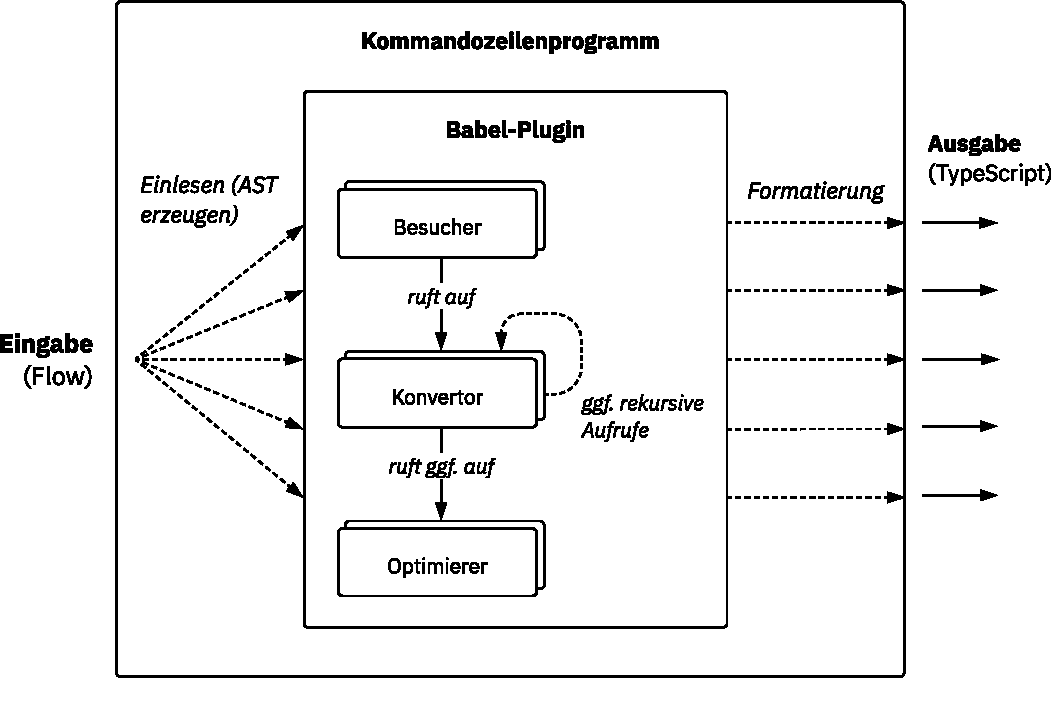
\includegraphics[width=\textwidth]{src/figures/architecture-overview.pdf}
        \end{figure}
      \end{columns}
    \end{frame}

    \begin{frame}[fragile]
      \frametitle{Spezialfälle (Auswahl)}
      \begin{columns}
        \column{\dimexpr\paperwidth-11mm}
          \begin{lstlisting}[
            basicstyle=\linespread{1.04}\footnotesize\ttfamily,
            numbers=none,
          ]
// Flow                               // TypeScript

type MaybeNull = ?null;               type MaybeNull = null | undefined;
                                      // (vs. null | null | undefined)

type FunctionType =                   type FunctionType =
  (string, arg: number) => mixed;       (p1: string, arg: number) => unknown;

function f(opt?: number = 10) {}      function f(opt: number = 10) {}

class C {                             class C
  constructor(): Date {                 constructor() {
    return new Date();                    return new Date();
  }                                     }
}                                     }
        \end{lstlisting}
      \end{columns}
    \end{frame}

  \section{Ergebnisse}
    \secframe{Ergebnisse und\secframebr Auswertung}

    % \begin{frame}
    %   \frametitle{Durchführung der Migration}
    %   \begin{itemize}
    %     \item Zwei Projekte von Spreadshirt wurden mit Hilfe des Transpilers erfolgreich migriert
    %     \item aber: daraufhin zahlreiche neue Typfehler
    %     \item manuelle Korrektur dieser Fehler notwendig
    %   \end{itemize}
    % \end{frame}

    \subsection{Technische Anforderungen}
      % \begin{frame}
      %   \LARGE\textbf{Erfüllung der technischen Anforderungen}
      % \end{frame}

      \begin{frame}
        \frametitle{A1\hspace{0.75em}Äquivalenz der Typ-Übersetzungen (1)}
        \begin{itemize}
          \item nahezu vollständig erzielt
          \item aber: einzelne Funktionen von Flow werden in TypeScript nicht unterstützt\\
            \smallskip
            $\Rightarrow$ Verlust von Typinformation hier unvermeidbar
          \item keine äquivalente TypeScript-Audrücke für 3 der 17 Hilfstypen von Flow gefunden\\
            \smallskip
            $\Rightarrow$ Ersetzung mit Typ \textit{any}
        \end{itemize}
      \end{frame}

      \begin{frame}[fragile]
        \frametitle{A1\hspace{0.75em}Äquivalenz der Typ-Übersetzungen (2)}
        \begin{columns}
          \column{\dimexpr\paperwidth-16mm}
          \textbf{Warnung bei Transformationen mit Typverlust}
          \vspace{1.5em}
          \begin{lstlisting}[emph={Warning},numbers=none]
Transpiling example.js...

  1 | // @flow
> 2 | const existentialType: * = f();
    |                       ^
  Warning:
    Flow's Existential Type (*) is not expressible in TypeScript.
    Therefore, it will be replaced with 'any'.
    See https://github.com/Microsoft/TypeScript/issues/14466.
            \end{lstlisting}
        \end{columns}

      \end{frame}

      \begin{frame}
        \frametitle{A1\hspace{0.75em}Vollständigkeit der Transformationen}
        \begin{itemize}
          \item wurde erzielt
          \item \textit{Vollständigkeit} durch AST-Spezifikation~\autocite{BABEL:PARSER_SPEC} von Babel präzise eingegrenzt
          \item Verifizierung durch 1022 Fixture-Tests\\(testgetriebene Entwicklung)
          \item außerdem: statische Überprüfung der Implementierung durch Typisierung von Babel
        \end{itemize}
      \end{frame}

      \begin{frame}
        \frametitle{A2\hspace{0.75em}Beibehaltung der Programmsemantik}
          \begin{itemize}
            \item Voraussetzung: Transpiler adressiert nur Flow-Typen,\\hat keine unbeabsichtigte Nebenwirkung
            \item Verifizierung dieser Bedingung durch Fixture-Tests
            \item Überprüfung der Semantik-Beibehaltung durch\\373 bzw. 326 Modultests der migrierten Projekte\\
              \smallskip
              $\Rightarrow$ keine Fehler, Anforderung scheint somit erfüllt
            \item aber: Testabdeckung bei 90,5\% bzw. lediglich 18,0\%
            \item \textbf{Nachtrag:} ein semantischer Fehler bei Umformung von Klassendekoratoren inzwischen erkannt
          \end{itemize}
      \end{frame}

      \begin{frame}
        \frametitle{A3\hspace{0.75em}Unterstützung von JavaScript- und JSX-Syntax}
        \begin{itemize}
          \item vollständige Unterstützung von ECMAScript 10 (2019) durch Babel
          \item Verarbeitung von vorläufiger JavaScript und JSX-Syntax mittels entsprechender Babel-Plugins
          \item Anforderung damit erfüllt
        \end{itemize}
      \end{frame}

      \begin{frame}[fragile]
        \frametitle{A4\hspace{0.75em}Verarbeitung gesamter Projektverzeichnisse}
        \begin{itemize}
          \item Umgesetztes Kommandozeilenprogramm ermöglicht Verarbeitung von Verzeichnissen (und von Einzeldateien)
          \item Flexible Ein- und Ausgrenzung von Eingabedateien durch Wildcard-Muster (\textit{glob patterns})
          \item Ausgabemodus durch Option steuerbar\\(Standardausgabe, Datei schreiben bzw. Original ersetzen)
        \end{itemize}

        \bigskip
        \begin{lstlisting}[numbers=none]
reflow \
  --dry-run \
  --exclude-pattern '**/tests/**/*.{js,jsx}' \
  src/
        \end{lstlisting}
      \end{frame}

      \begin{frame}
        \frametitle{A5\hspace{0.75em}Originalgetreue Formatierung der Ausgabe}
        \begin{itemize}
          \item ursprüngliche Quelltextformatierung geht durch AST-Transformation verloren
          \item deshalb: Formatierungsroutine auf Basis von\\\textit{Prettier}~\autocite{SOFTWARE:PRETTIER} implementiert
          \item Manuelle Überprüfung der korrekten Formatierung\\der Ausgabe in zwei Projekten:\\
            \medskip
            {
              \footnotesize
              \begin{tabu} to \textwidth {@{}lr@{}}
                Projekt Components & 3,5\% Fehlerrate \\
                Projekt Helios     & 5,9\% Fehlerrate \\
              \end{tabu}
            }
          \item Fazit: vereinzelt Fehler, aber originalgetreue\\Formatierung in 95,3\% der Fälle
        \end{itemize}
      \end{frame}

    \subsection{Ziele}
      % \begin{frame}
      %   \LARGE\textbf{Erfüllung der Zielvorgaben}
      % \end{frame}

      \begin{frame}
        \frametitle{Z1\hspace{0.75em}Erkennung weiterer Typ- und Programmfehler}

        Nach Migration 543 bzw. 404 neue nicht-strikte Typfehler in Projekten Components bzw. Helios:\\[1em]
        {
          \footnotesize
          \begin{tabu} to \textwidth {@{}rrX@{}}
            \midrule
            \rowfont[l]{\bfseries} Anzahl & Fehler & Beschreibung \\
            \midrule
            272	& TS2322 & Typ \codei{x} ist Typ \codei{y} nicht zuweisbar \\
            205	& TS2307 & Modul \codei{x} kann nicht gefunden werden \\
            128	& TS2345 & Argument mit Typ \codei{x} ist Param. mit Typ \codei{y} nicht zuweisbar \\
            94	& TS2339 & Attribut \codei{x} existiert nicht in Typ \codei{y} \\
            72	& TS2605 & Modul \codei{x} exportiert kein Element \codei{y} \\
            % 54	& TS2304 & Name \codei{x} kann nicht gefunden werden \\
            % 25	& TS2538 & Typ \codei{x} darf nicht als Index-Typ verwendet werden \\
            % 23	& TS2741 & Attribut \codei{x} fehlt in Typ \codei{y}, wird aber von Typ \codei{z} erwartet \\
            \midrule
          \end{tabu}
        }
        \\[1em]
        aber: Großteil der Typverletzungen stellen keine Programmfehler dar
      \end{frame}

      \begin{frame}
        \frametitle{Z1\hspace{0.75em}Erkennung weiterer Typ- und Programmfehler}

        \begin{block}{Ursachen neu aufgetrener Typfehler}
          \begin{itemize}
            \item Prinzipielle Unterschiede von Flow und TypeScript
            \item Integration externer Typdefinitionen
            \item Unzulänglichkeiten der vorherigen Typisierung mit Flow
          \end{itemize}
        \end{block}
        \smallskip
        \begin{block}{Von TypeScript aufgedeckte Programmfehler}
          \begin{itemize}
            \item Zusätzliche Objektattribute bei Funktionsargumenten
            \item Fehlerhafte Verwendung von React-Komponenten
            \item Falscher Argumenttyp bei Funktionsaufrufen
          \end{itemize}
        \end{block}
      \end{frame}

      \begin{frame}
        \frametitle{Z2\hspace{0.75em}Unterstützung externer Bibliotheken (1)}
        Zwei Projekte stellen Typdefinitionen für JavaScript-Bibliotheken bereit:\\[1.5em]
        {
          \footnotesize
          \begin{tabu} to \textwidth {@{}lrrrrl@{}}
            \midrule
            \rowfont{\bfseries} Projekt & Typdef. & Commits & Beitragende & Sterne & {} \\
            \midrule
            flow-typed      &  628 &  520 &  201 &  3.400 & \autocite{FLOW_TYPED} \\
            DefinitelyTyped & 6202 & 8188 & 1785 & 25.000 & \autocite{DEFINITELY_TYPED} \\
            \midrule
          \end{tabu}
          \\[1em]
          Stand: Oktober 2019 -- Commits und Beitragende im Jahresmittel
        }
      \end{frame}

      \begin{frame}
        \frametitle{Z2\hspace{0.75em}Unterstützung externer Bibliotheken (2)}
        Untersuchung der 15 am häufigsten eingesetzten\\Bibliotheken in migrierten Projekten:\\[1em]
        {
          \footnotesize
          \begin{tabu} to \textwidth {@{}lrrl@{}}
            \midrule
            \rowfont{\bfseries} {} & Flow & TypeScript \\
            \midrule
            Keine Typdefinition verfügbar &  4 &  1 \\
            In Paket integriert           &  1 &  3 \\
            Separat gepflegt              & 10 & 11 \\
            \midrule
            Abweichung von Hauptversion   &  0 &  2 \\
            Abweichung von Nebenversion   &  ? &  3 \\
            \midrule
          \end{tabu}
          \\[.75em]
          Stand: November 2019
        }
        \\[1.25em]
        aber: für diese Auswahl von Bibliotheken nur\\geringfügige Vorteile bei TypeScript
      \end{frame}

      \begin{frame}
        \frametitle{Z3\hspace{0.75em}Performance -- Vollständige Typüberprüfung (1)}
        % GNUPLOT: LaTeX picture with Postscript
\begingroup
  \makeatletter
  \providecommand\color[2][]{%
    \GenericError{(gnuplot) \space\space\space\@spaces}{%
      Package color not loaded in conjunction with
      terminal option `colourtext'%
    }{See the gnuplot documentation for explanation.%
    }{Either use 'blacktext' in gnuplot or load the package
      color.sty in LaTeX.}%
    \renewcommand\color[2][]{}%
  }%
  \providecommand\includegraphics[2][]{%
    \GenericError{(gnuplot) \space\space\space\@spaces}{%
      Package graphicx or graphics not loaded%
    }{See the gnuplot documentation for explanation.%
    }{The gnuplot epslatex terminal needs graphicx.sty or graphics.sty.}%
    \renewcommand\includegraphics[2][]{}%
  }%
  \providecommand\rotatebox[2]{#2}%
  \@ifundefined{ifGPcolor}{%
    \newif\ifGPcolor
    \GPcolortrue
  }{}%
  \@ifundefined{ifGPblacktext}{%
    \newif\ifGPblacktext
    \GPblacktexttrue
  }{}%
  % define a \g@addto@macro without @ in the name:
  \let\gplgaddtomacro\g@addto@macro
  % define empty templates for all commands taking text:
  \gdef\gplbacktext{}%
  \gdef\gplfronttext{}%
  \makeatother
  \ifGPblacktext
    % no textcolor at all
    \def\colorrgb#1{}%
    \def\colorgray#1{}%
  \else
    % gray or color?
    \ifGPcolor
      \def\colorrgb#1{\color[rgb]{#1}}%
      \def\colorgray#1{\color[gray]{#1}}%
      \expandafter\def\csname LTw\endcsname{\color{white}}%
      \expandafter\def\csname LTb\endcsname{\color{black}}%
      \expandafter\def\csname LTa\endcsname{\color{black}}%
      \expandafter\def\csname LT0\endcsname{\color[rgb]{1,0,0}}%
      \expandafter\def\csname LT1\endcsname{\color[rgb]{0,1,0}}%
      \expandafter\def\csname LT2\endcsname{\color[rgb]{0,0,1}}%
      \expandafter\def\csname LT3\endcsname{\color[rgb]{1,0,1}}%
      \expandafter\def\csname LT4\endcsname{\color[rgb]{0,1,1}}%
      \expandafter\def\csname LT5\endcsname{\color[rgb]{1,1,0}}%
      \expandafter\def\csname LT6\endcsname{\color[rgb]{0,0,0}}%
      \expandafter\def\csname LT7\endcsname{\color[rgb]{1,0.3,0}}%
      \expandafter\def\csname LT8\endcsname{\color[rgb]{0.5,0.5,0.5}}%
    \else
      % gray
      \def\colorrgb#1{\color{black}}%
      \def\colorgray#1{\color[gray]{#1}}%
      \expandafter\def\csname LTw\endcsname{\color{white}}%
      \expandafter\def\csname LTb\endcsname{\color{black}}%
      \expandafter\def\csname LTa\endcsname{\color{black}}%
      \expandafter\def\csname LT0\endcsname{\color{black}}%
      \expandafter\def\csname LT1\endcsname{\color{black}}%
      \expandafter\def\csname LT2\endcsname{\color{black}}%
      \expandafter\def\csname LT3\endcsname{\color{black}}%
      \expandafter\def\csname LT4\endcsname{\color{black}}%
      \expandafter\def\csname LT5\endcsname{\color{black}}%
      \expandafter\def\csname LT6\endcsname{\color{black}}%
      \expandafter\def\csname LT7\endcsname{\color{black}}%
      \expandafter\def\csname LT8\endcsname{\color{black}}%
    \fi
  \fi
    \setlength{\unitlength}{0.0500bp}%
    \ifx\gptboxheight\undefined%
      \newlength{\gptboxheight}%
      \newlength{\gptboxwidth}%
      \newsavebox{\gptboxtext}%
    \fi%
    \setlength{\fboxrule}{0.5pt}%
    \setlength{\fboxsep}{1pt}%
\begin{picture}(6640.00,3940.00)%
    \gplgaddtomacro\gplbacktext{%
      \footnotesize%
      \csname LTb\endcsname%%
      \put(596,652){\makebox(0,0)[r]{\strut{}$2$}}%
      \csname LTb\endcsname%%
      \put(596,1090){\makebox(0,0)[r]{\strut{}$4$}}%
      \csname LTb\endcsname%%
      \put(596,1527){\makebox(0,0)[r]{\strut{}$6$}}%
      \csname LTb\endcsname%%
      \put(596,1965){\makebox(0,0)[r]{\strut{}$8$}}%
      \csname LTb\endcsname%%
      \put(596,2402){\makebox(0,0)[r]{\strut{}$10$}}%
      \csname LTb\endcsname%%
      \put(596,2840){\makebox(0,0)[r]{\strut{}$12$}}%
      \csname LTb\endcsname%%
      \put(596,3277){\makebox(0,0)[r]{\strut{}$14$}}%
      \csname LTb\endcsname%%
      \put(596,3715){\makebox(0,0)[r]{\strut{}$16$}}%
      \csname LTb\endcsname%%
      \put(1827,448){\makebox(0,0){\strut{}A}}%
      \csname LTb\endcsname%%
      \put(2946,448){\makebox(0,0){\strut{}B}}%
      \csname LTb\endcsname%%
      \put(4065,448){\makebox(0,0){\strut{}C}}%
      \csname LTb\endcsname%%
      \put(5184,448){\makebox(0,0){\strut{}D}}%
    }%
    \gplgaddtomacro\gplfronttext{%
      \csname LTb\endcsname%%
      \put(74,2183){\rotatebox{-270}{\makebox(0,0){\strut{}\footnotesize durchschnittliche Laufzeit in s}}}%
      \csname LTb\endcsname%%
      \put(3505,142){\makebox(0,0){\strut{}\footnotesize Testsystem}}%
      \csname LTb\endcsname%%
      \put(3505,3409){\makebox(0,0){\strut{}\footnotesize\bfseries Components}}%
      \csname LTb\endcsname%%
      \put(5438,3430){\makebox(0,0)[r]{\strut{}\scriptsize Flow}}%
      \csname LTb\endcsname%%
      \put(5438,3226){\makebox(0,0)[r]{\strut{}\scriptsize TypeScript}}%
    }%
    \gplbacktext
    \put(0,0){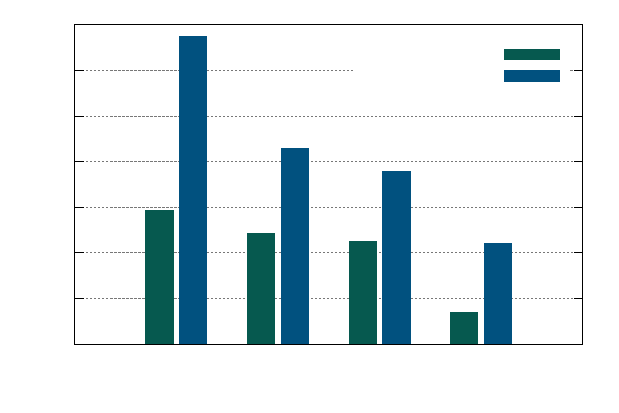
\includegraphics{src/plots/complete/components-plot}}%
    \gplfronttext
  \end{picture}%
\endgroup

      \end{frame}

      \begin{frame}
        \frametitle{Z3\hspace{0.75em}Performance -- Vollständige Typüberprüfung (2)}
        % GNUPLOT: LaTeX picture with Postscript
\begingroup
  \makeatletter
  \providecommand\color[2][]{%
    \GenericError{(gnuplot) \space\space\space\@spaces}{%
      Package color not loaded in conjunction with
      terminal option `colourtext'%
    }{See the gnuplot documentation for explanation.%
    }{Either use 'blacktext' in gnuplot or load the package
      color.sty in LaTeX.}%
    \renewcommand\color[2][]{}%
  }%
  \providecommand\includegraphics[2][]{%
    \GenericError{(gnuplot) \space\space\space\@spaces}{%
      Package graphicx or graphics not loaded%
    }{See the gnuplot documentation for explanation.%
    }{The gnuplot epslatex terminal needs graphicx.sty or graphics.sty.}%
    \renewcommand\includegraphics[2][]{}%
  }%
  \providecommand\rotatebox[2]{#2}%
  \@ifundefined{ifGPcolor}{%
    \newif\ifGPcolor
    \GPcolortrue
  }{}%
  \@ifundefined{ifGPblacktext}{%
    \newif\ifGPblacktext
    \GPblacktexttrue
  }{}%
  % define a \g@addto@macro without @ in the name:
  \let\gplgaddtomacro\g@addto@macro
  % define empty templates for all commands taking text:
  \gdef\gplbacktext{}%
  \gdef\gplfronttext{}%
  \makeatother
  \ifGPblacktext
    % no textcolor at all
    \def\colorrgb#1{}%
    \def\colorgray#1{}%
  \else
    % gray or color?
    \ifGPcolor
      \def\colorrgb#1{\color[rgb]{#1}}%
      \def\colorgray#1{\color[gray]{#1}}%
      \expandafter\def\csname LTw\endcsname{\color{white}}%
      \expandafter\def\csname LTb\endcsname{\color{black}}%
      \expandafter\def\csname LTa\endcsname{\color{black}}%
      \expandafter\def\csname LT0\endcsname{\color[rgb]{1,0,0}}%
      \expandafter\def\csname LT1\endcsname{\color[rgb]{0,1,0}}%
      \expandafter\def\csname LT2\endcsname{\color[rgb]{0,0,1}}%
      \expandafter\def\csname LT3\endcsname{\color[rgb]{1,0,1}}%
      \expandafter\def\csname LT4\endcsname{\color[rgb]{0,1,1}}%
      \expandafter\def\csname LT5\endcsname{\color[rgb]{1,1,0}}%
      \expandafter\def\csname LT6\endcsname{\color[rgb]{0,0,0}}%
      \expandafter\def\csname LT7\endcsname{\color[rgb]{1,0.3,0}}%
      \expandafter\def\csname LT8\endcsname{\color[rgb]{0.5,0.5,0.5}}%
    \else
      % gray
      \def\colorrgb#1{\color{black}}%
      \def\colorgray#1{\color[gray]{#1}}%
      \expandafter\def\csname LTw\endcsname{\color{white}}%
      \expandafter\def\csname LTb\endcsname{\color{black}}%
      \expandafter\def\csname LTa\endcsname{\color{black}}%
      \expandafter\def\csname LT0\endcsname{\color{black}}%
      \expandafter\def\csname LT1\endcsname{\color{black}}%
      \expandafter\def\csname LT2\endcsname{\color{black}}%
      \expandafter\def\csname LT3\endcsname{\color{black}}%
      \expandafter\def\csname LT4\endcsname{\color{black}}%
      \expandafter\def\csname LT5\endcsname{\color{black}}%
      \expandafter\def\csname LT6\endcsname{\color{black}}%
      \expandafter\def\csname LT7\endcsname{\color{black}}%
      \expandafter\def\csname LT8\endcsname{\color{black}}%
    \fi
  \fi
    \setlength{\unitlength}{0.0500bp}%
    \ifx\gptboxheight\undefined%
      \newlength{\gptboxheight}%
      \newlength{\gptboxwidth}%
      \newsavebox{\gptboxtext}%
    \fi%
    \setlength{\fboxrule}{0.5pt}%
    \setlength{\fboxsep}{1pt}%
\begin{picture}(6640.00,3940.00)%
    \gplgaddtomacro\gplbacktext{%
      \footnotesize%
      \csname LTb\endcsname%%
      \put(596,652){\makebox(0,0)[r]{\strut{}$4$}}%
      \csname LTb\endcsname%%
      \put(596,958){\makebox(0,0)[r]{\strut{}$5$}}%
      \csname LTb\endcsname%%
      \put(596,1265){\makebox(0,0)[r]{\strut{}$6$}}%
      \csname LTb\endcsname%%
      \put(596,1571){\makebox(0,0)[r]{\strut{}$7$}}%
      \csname LTb\endcsname%%
      \put(596,1877){\makebox(0,0)[r]{\strut{}$8$}}%
      \csname LTb\endcsname%%
      \put(596,2184){\makebox(0,0)[r]{\strut{}$9$}}%
      \csname LTb\endcsname%%
      \put(596,2490){\makebox(0,0)[r]{\strut{}$10$}}%
      \csname LTb\endcsname%%
      \put(596,2796){\makebox(0,0)[r]{\strut{}$11$}}%
      \csname LTb\endcsname%%
      \put(596,3102){\makebox(0,0)[r]{\strut{}$12$}}%
      \csname LTb\endcsname%%
      \put(596,3409){\makebox(0,0)[r]{\strut{}$13$}}%
      \csname LTb\endcsname%%
      \put(596,3715){\makebox(0,0)[r]{\strut{}$14$}}%
      \csname LTb\endcsname%%
      \put(1827,448){\makebox(0,0){\strut{}A}}%
      \csname LTb\endcsname%%
      \put(2946,448){\makebox(0,0){\strut{}B}}%
      \csname LTb\endcsname%%
      \put(4065,448){\makebox(0,0){\strut{}C}}%
      \csname LTb\endcsname%%
      \put(5184,448){\makebox(0,0){\strut{}D}}%
    }%
    \gplgaddtomacro\gplfronttext{%
      \csname LTb\endcsname%%
      \put(74,2183){\rotatebox{-270}{\makebox(0,0){\strut{}\footnotesize durchschnittliche Laufzeit in s}}}%
      \csname LTb\endcsname%%
      \put(3505,142){\makebox(0,0){\strut{}\footnotesize Testsystem}}%
      \csname LTb\endcsname%%
      \put(3505,3409){\makebox(0,0){\strut{}\footnotesize\bfseries Helios}}%
      \csname LTb\endcsname%%
      \put(5438,3430){\makebox(0,0)[r]{\strut{}\footnotesize Flow}}%
      \csname LTb\endcsname%%
      \put(5438,3226){\makebox(0,0)[r]{\strut{}\footnotesize TypeScript}}%
    }%
    \gplbacktext
    \put(0,0){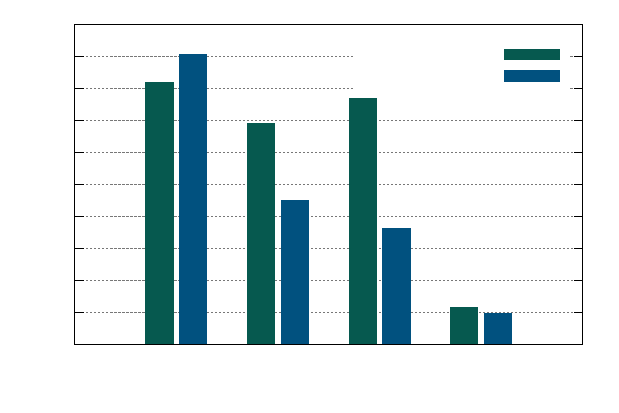
\includegraphics{src/plots/complete/helios-plot}}%
    \gplfronttext
  \end{picture}%
\endgroup

      \end{frame}

      \begin{frame}
        \frametitle{Z3\hspace{0.75em}Performance -- Einfluss der Parallelisierung (1)}
        % GNUPLOT: LaTeX picture with Postscript
\begingroup
  \makeatletter
  \providecommand\color[2][]{%
    \GenericError{(gnuplot) \space\space\space\@spaces}{%
      Package color not loaded in conjunction with
      terminal option `colourtext'%
    }{See the gnuplot documentation for explanation.%
    }{Either use 'blacktext' in gnuplot or load the package
      color.sty in LaTeX.}%
    \renewcommand\color[2][]{}%
  }%
  \providecommand\includegraphics[2][]{%
    \GenericError{(gnuplot) \space\space\space\@spaces}{%
      Package graphicx or graphics not loaded%
    }{See the gnuplot documentation for explanation.%
    }{The gnuplot epslatex terminal needs graphicx.sty or graphics.sty.}%
    \renewcommand\includegraphics[2][]{}%
  }%
  \providecommand\rotatebox[2]{#2}%
  \@ifundefined{ifGPcolor}{%
    \newif\ifGPcolor
    \GPcolortrue
  }{}%
  \@ifundefined{ifGPblacktext}{%
    \newif\ifGPblacktext
    \GPblacktexttrue
  }{}%
  % define a \g@addto@macro without @ in the name:
  \let\gplgaddtomacro\g@addto@macro
  % define empty templates for all commands taking text:
  \gdef\gplbacktext{}%
  \gdef\gplfronttext{}%
  \makeatother
  \ifGPblacktext
    % no textcolor at all
    \def\colorrgb#1{}%
    \def\colorgray#1{}%
  \else
    % gray or color?
    \ifGPcolor
      \def\colorrgb#1{\color[rgb]{#1}}%
      \def\colorgray#1{\color[gray]{#1}}%
      \expandafter\def\csname LTw\endcsname{\color{white}}%
      \expandafter\def\csname LTb\endcsname{\color{black}}%
      \expandafter\def\csname LTa\endcsname{\color{black}}%
      \expandafter\def\csname LT0\endcsname{\color[rgb]{1,0,0}}%
      \expandafter\def\csname LT1\endcsname{\color[rgb]{0,1,0}}%
      \expandafter\def\csname LT2\endcsname{\color[rgb]{0,0,1}}%
      \expandafter\def\csname LT3\endcsname{\color[rgb]{1,0,1}}%
      \expandafter\def\csname LT4\endcsname{\color[rgb]{0,1,1}}%
      \expandafter\def\csname LT5\endcsname{\color[rgb]{1,1,0}}%
      \expandafter\def\csname LT6\endcsname{\color[rgb]{0,0,0}}%
      \expandafter\def\csname LT7\endcsname{\color[rgb]{1,0.3,0}}%
      \expandafter\def\csname LT8\endcsname{\color[rgb]{0.5,0.5,0.5}}%
    \else
      % gray
      \def\colorrgb#1{\color{black}}%
      \def\colorgray#1{\color[gray]{#1}}%
      \expandafter\def\csname LTw\endcsname{\color{white}}%
      \expandafter\def\csname LTb\endcsname{\color{black}}%
      \expandafter\def\csname LTa\endcsname{\color{black}}%
      \expandafter\def\csname LT0\endcsname{\color{black}}%
      \expandafter\def\csname LT1\endcsname{\color{black}}%
      \expandafter\def\csname LT2\endcsname{\color{black}}%
      \expandafter\def\csname LT3\endcsname{\color{black}}%
      \expandafter\def\csname LT4\endcsname{\color{black}}%
      \expandafter\def\csname LT5\endcsname{\color{black}}%
      \expandafter\def\csname LT6\endcsname{\color{black}}%
      \expandafter\def\csname LT7\endcsname{\color{black}}%
      \expandafter\def\csname LT8\endcsname{\color{black}}%
    \fi
  \fi
    \setlength{\unitlength}{0.0500bp}%
    \ifx\gptboxheight\undefined%
      \newlength{\gptboxheight}%
      \newlength{\gptboxwidth}%
      \newsavebox{\gptboxtext}%
    \fi%
    \setlength{\fboxrule}{0.5pt}%
    \setlength{\fboxsep}{1pt}%
\begin{picture}(6480.00,3940.00)%
    \gplgaddtomacro\gplbacktext{%
      \footnotesize%
      \csname LTb\endcsname%%
      \put(596,652){\makebox(0,0)[r]{\strut{}$3$}}%
      \csname LTb\endcsname%%
      \put(596,1035){\makebox(0,0)[r]{\strut{}$4$}}%
      \csname LTb\endcsname%%
      \put(596,1418){\makebox(0,0)[r]{\strut{}$5$}}%
      \csname LTb\endcsname%%
      \put(596,1801){\makebox(0,0)[r]{\strut{}$6$}}%
      \csname LTb\endcsname%%
      \put(596,2184){\makebox(0,0)[r]{\strut{}$7$}}%
      \csname LTb\endcsname%%
      \put(596,2566){\makebox(0,0)[r]{\strut{}$8$}}%
      \csname LTb\endcsname%%
      \put(596,2949){\makebox(0,0)[r]{\strut{}$9$}}%
      \csname LTb\endcsname%%
      \put(596,3332){\makebox(0,0)[r]{\strut{}$10$}}%
      \csname LTb\endcsname%%
      \put(596,3715){\makebox(0,0)[r]{\strut{}$11$}}%
      \csname LTb\endcsname%%
      \put(1312,448){\makebox(0,0){\strut{}1}}%
      \csname LTb\endcsname%%
      \put(1916,448){\makebox(0,0){\strut{}2}}%
      \csname LTb\endcsname%%
      \put(2520,448){\makebox(0,0){\strut{}3}}%
      \csname LTb\endcsname%%
      \put(3124,448){\makebox(0,0){\strut{}4}}%
      \csname LTb\endcsname%%
      \put(3727,448){\makebox(0,0){\strut{}5}}%
      \csname LTb\endcsname%%
      \put(4331,448){\makebox(0,0){\strut{}6}}%
      \csname LTb\endcsname%%
      \put(4935,448){\makebox(0,0){\strut{}7}}%
      \csname LTb\endcsname%%
      \put(5539,448){\makebox(0,0){\strut{}8}}%
    }%
    \gplgaddtomacro\gplfronttext{%
      \csname LTb\endcsname%%
      \put(74,2183){\rotatebox{-270}{\makebox(0,0){\strut{}\footnotesize durchschnittliche Laufzeit in s}}}%
      \csname LTb\endcsname%%
      \put(3425,142){\makebox(0,0){\strut{}\footnotesize Anzahl verfügbarer Prozessorkerne}}%
      \csname LTb\endcsname%%
      \put(3425,3409){\makebox(0,0){\strut{}\footnotesize\bfseries Components}}%
      \csname LTb\endcsname%%
      \put(5278,3430){\makebox(0,0)[r]{\strut{}\scriptsize Flow}}%
      \csname LTb\endcsname%%
      \put(5278,3226){\makebox(0,0)[r]{\strut{}\scriptsize TypeScript}}%
    }%
    \gplbacktext
    \put(0,0){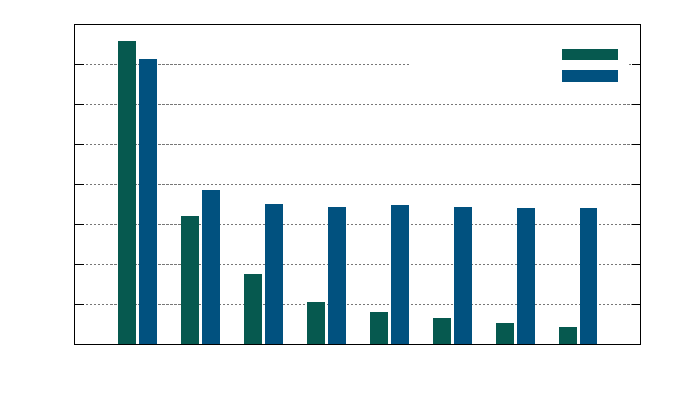
\includegraphics{src/plots/cores/components-plot}}%
    \gplfronttext
  \end{picture}%
\endgroup

      \end{frame}

      \begin{frame}
        \frametitle{Z3\hspace{0.75em}Performance -- Einfluss der Parallelisierung (2)}
        % GNUPLOT: LaTeX picture with Postscript
\begingroup
  \makeatletter
  \providecommand\color[2][]{%
    \GenericError{(gnuplot) \space\space\space\@spaces}{%
      Package color not loaded in conjunction with
      terminal option `colourtext'%
    }{See the gnuplot documentation for explanation.%
    }{Either use 'blacktext' in gnuplot or load the package
      color.sty in LaTeX.}%
    \renewcommand\color[2][]{}%
  }%
  \providecommand\includegraphics[2][]{%
    \GenericError{(gnuplot) \space\space\space\@spaces}{%
      Package graphicx or graphics not loaded%
    }{See the gnuplot documentation for explanation.%
    }{The gnuplot epslatex terminal needs graphicx.sty or graphics.sty.}%
    \renewcommand\includegraphics[2][]{}%
  }%
  \providecommand\rotatebox[2]{#2}%
  \@ifundefined{ifGPcolor}{%
    \newif\ifGPcolor
    \GPcolortrue
  }{}%
  \@ifundefined{ifGPblacktext}{%
    \newif\ifGPblacktext
    \GPblacktexttrue
  }{}%
  % define a \g@addto@macro without @ in the name:
  \let\gplgaddtomacro\g@addto@macro
  % define empty templates for all commands taking text:
  \gdef\gplbacktext{}%
  \gdef\gplfronttext{}%
  \makeatother
  \ifGPblacktext
    % no textcolor at all
    \def\colorrgb#1{}%
    \def\colorgray#1{}%
  \else
    % gray or color?
    \ifGPcolor
      \def\colorrgb#1{\color[rgb]{#1}}%
      \def\colorgray#1{\color[gray]{#1}}%
      \expandafter\def\csname LTw\endcsname{\color{white}}%
      \expandafter\def\csname LTb\endcsname{\color{black}}%
      \expandafter\def\csname LTa\endcsname{\color{black}}%
      \expandafter\def\csname LT0\endcsname{\color[rgb]{1,0,0}}%
      \expandafter\def\csname LT1\endcsname{\color[rgb]{0,1,0}}%
      \expandafter\def\csname LT2\endcsname{\color[rgb]{0,0,1}}%
      \expandafter\def\csname LT3\endcsname{\color[rgb]{1,0,1}}%
      \expandafter\def\csname LT4\endcsname{\color[rgb]{0,1,1}}%
      \expandafter\def\csname LT5\endcsname{\color[rgb]{1,1,0}}%
      \expandafter\def\csname LT6\endcsname{\color[rgb]{0,0,0}}%
      \expandafter\def\csname LT7\endcsname{\color[rgb]{1,0.3,0}}%
      \expandafter\def\csname LT8\endcsname{\color[rgb]{0.5,0.5,0.5}}%
    \else
      % gray
      \def\colorrgb#1{\color{black}}%
      \def\colorgray#1{\color[gray]{#1}}%
      \expandafter\def\csname LTw\endcsname{\color{white}}%
      \expandafter\def\csname LTb\endcsname{\color{black}}%
      \expandafter\def\csname LTa\endcsname{\color{black}}%
      \expandafter\def\csname LT0\endcsname{\color{black}}%
      \expandafter\def\csname LT1\endcsname{\color{black}}%
      \expandafter\def\csname LT2\endcsname{\color{black}}%
      \expandafter\def\csname LT3\endcsname{\color{black}}%
      \expandafter\def\csname LT4\endcsname{\color{black}}%
      \expandafter\def\csname LT5\endcsname{\color{black}}%
      \expandafter\def\csname LT6\endcsname{\color{black}}%
      \expandafter\def\csname LT7\endcsname{\color{black}}%
      \expandafter\def\csname LT8\endcsname{\color{black}}%
    \fi
  \fi
    \setlength{\unitlength}{0.0500bp}%
    \ifx\gptboxheight\undefined%
      \newlength{\gptboxheight}%
      \newlength{\gptboxwidth}%
      \newsavebox{\gptboxtext}%
    \fi%
    \setlength{\fboxrule}{0.5pt}%
    \setlength{\fboxsep}{1pt}%
\begin{picture}(6640.00,3940.00)%
    \gplgaddtomacro\gplbacktext{%
      \footnotesize%
      \csname LTb\endcsname%%
      \put(596,652){\makebox(0,0)[r]{\strut{}$4$}}%
      \csname LTb\endcsname%%
      \put(596,1090){\makebox(0,0)[r]{\strut{}$6$}}%
      \csname LTb\endcsname%%
      \put(596,1527){\makebox(0,0)[r]{\strut{}$8$}}%
      \csname LTb\endcsname%%
      \put(596,1965){\makebox(0,0)[r]{\strut{}$10$}}%
      \csname LTb\endcsname%%
      \put(596,2402){\makebox(0,0)[r]{\strut{}$12$}}%
      \csname LTb\endcsname%%
      \put(596,2840){\makebox(0,0)[r]{\strut{}$14$}}%
      \csname LTb\endcsname%%
      \put(596,3277){\makebox(0,0)[r]{\strut{}$16$}}%
      \csname LTb\endcsname%%
      \put(596,3715){\makebox(0,0)[r]{\strut{}$18$}}%
      \csname LTb\endcsname%%
      \put(1330,448){\makebox(0,0){\strut{}1}}%
      \csname LTb\endcsname%%
      \put(1951,448){\makebox(0,0){\strut{}2}}%
      \csname LTb\endcsname%%
      \put(2573,448){\makebox(0,0){\strut{}3}}%
      \csname LTb\endcsname%%
      \put(3195,448){\makebox(0,0){\strut{}4}}%
      \csname LTb\endcsname%%
      \put(3816,448){\makebox(0,0){\strut{}5}}%
      \csname LTb\endcsname%%
      \put(4438,448){\makebox(0,0){\strut{}6}}%
      \csname LTb\endcsname%%
      \put(5060,448){\makebox(0,0){\strut{}7}}%
      \csname LTb\endcsname%%
      \put(5681,448){\makebox(0,0){\strut{}8}}%
    }%
    \gplgaddtomacro\gplfronttext{%
      \csname LTb\endcsname%%
      \put(74,2183){\rotatebox{-270}{\makebox(0,0){\strut{}\footnotesize durchschnittliche Laufzeit in s}}}%
      \csname LTb\endcsname%%
      \put(3505,142){\makebox(0,0){\strut{}\footnotesize Anzahl verfügbarer Prozessorkerne}}%
      \csname LTb\endcsname%%
      \put(3505,3409){\makebox(0,0){\strut{}\footnotesize\bfseries Helios}}%
      \csname LTb\endcsname%%
      \put(5438,3430){\makebox(0,0)[r]{\strut{}\footnotesize Flow}}%
      \csname LTb\endcsname%%
      \put(5438,3226){\makebox(0,0)[r]{\strut{}\footnotesize TypeScript}}%
    }%
    \gplbacktext
    \put(0,0){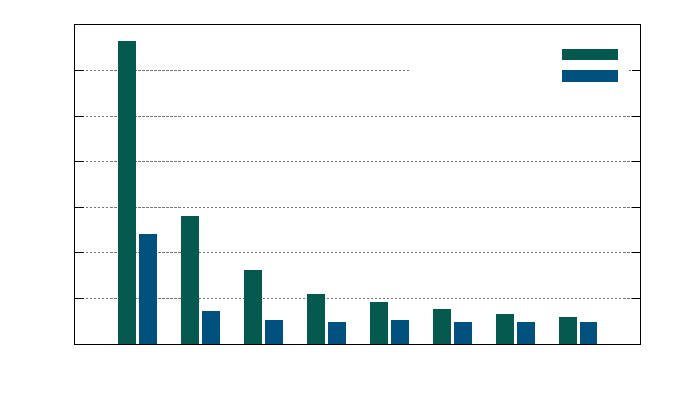
\includegraphics{src/plots/cores/helios-plot}}%
    \gplfronttext
  \end{picture}%
\endgroup

      \end{frame}

      \begin{frame}
        \frametitle{Z4\hspace{0.75em}Zukunftssicherheit und Transparenz}
        \begin{itemize}
          \item Problem: Verunsicherung bezüglich der Zukunft von Flow
          \item Kommunikation laut eigener Aussage zuletzt ungenügend~\autocite{FLOW:UPDATE_2019}
          \item öffentlich einsehbarer Projektplan (\textit{Roadmap}) nur bei TypeScript verfügbar
          \item Untersuchung wie schnell Fehlerberichte (\textit{Issues}) auf GitHub im Median geschlossen wurden:\\
            \vspace{.5em}
            {
              \footnotesize
              \begin{tabu}{@{}lrr@{}}
                Flow & 11,6 Tage & 3.800 Einträge \\
                TypeScript & 6,6 Tage & 20.000 Einträge \\
              \end{tabu}
            }
          \item Fazit: Entwicklung von TypeScript\\tatsächlich transparenter
        \end{itemize}
      \end{frame}

  \section{Zusammenfassung}
    \secframe{Zusammenfassung}

    \begin{frame}
      \frametitle{Zusammenfassung}
      \textbf{Erfüllung der technischen Anforderungen}\\[1em]
      {
        \renewcommand{\arraystretch}{1.4}
        \begin{tabu} to \textwidth {@{}lX@{}}
          \textbf{A1} & Äquivalente und vollständige Übersetzung der Flow-Typen \\
          \textbf{A2} & Beibehaltung der Programmsemantik \\
          \textbf{A3} & Unterstützung aktueller und vorläufiger JavaScript- sowie JSX-Syntax (React) \\
          \textbf{A4} & Verarbeitung gesamter Projektverzeichnisse \\
          \textbf{A5} & Originalgetreue Formatierung der Ausgabe \\
        \end{tabu}
      }
    \end{frame}

    \begin{frame}
      \frametitle{Zusammenfassung}
      \textbf{Erfüllung der Ziele}\\[1em]
      {
        \renewcommand{\arraystretch}{1.4}
        \begin{tabu} to \textwidth {@{}lX@{}}
          \textbf{Z1} & Erkennung weiterer Typ- und Programmfehler \\
          \textbf{Z2} & Unterstützung externer Bibliotheken \\
          \textbf{Z3} & Performance der Typüberprüfungen \\
          \textbf{Z4} & Zukunftssicherheit und Transparenz der Technologie \\
        \end{tabu}
      }
    \end{frame}

  \appendix
    \begin{frame}[noframenumbering,plain]
      % empty
    \end{frame}

  \section{Backup}
    \setbeamertemplate{footline}{}

    \begin{frame}[noframenumbering]
      \frametitle{Evaluation bestehender Werkzeuge}
      {
  \footnotesize
  \begin{tabu} to \textwidth {@{}lllccccccrrX@{}}
    \midrule
    Werkzeug & Typ & Format & Erw. & ES10 & ES10+ & Flow & TS & JSX \\
    \midrule
    Acorn     & P  &  ESTree  & \pie{2} & \pie{2} & \pie{1} & \pie{0} & \pie{0} & \pie{2} \\ % 2012
    Astring   & G  &  ESTree  & \pie{2} & \pie{2} & \pie{1} & \pie{0} & \pie{0} & \pie{0} \\ % 2015
    Babel     & PG &  Babel   & \pie{2} & \pie{2} & \pie{2} & \pie{2} & \pie{2} & \pie{2} \\ % 2014
    Escodegen & G  &  ESTree  & \pie{0} & \pie{0} & \pie{0} & \pie{0} & \pie{0} & \pie{0} \\ % 2012
    Esprima   & P  &  ESTree  & \pie{0} & \pie{1} & \pie{0} & \pie{0} & \pie{0} & \pie{1} \\ % 2011
    Recast    & PG &  diverse & \pie{2} & \pie{2} & \pie{2} & \pie{2} & \pie{2} & \pie{2} \\ % 2012
    \midrule
  \end{tabu}

  \vspace{5mm}
  \begin{columns}[T]
    \begin{column}{0.4\textwidth}
      {
        \renewcommand{\arraystretch}{1.1}
        \begin{tabular}{@{}ll@{}}
          P & Parser\\
          G & Codegenerator\\
          \pie{0} & keine Unterstützung\\
          \pie{1} & teilweise Unterstützung\\
          \pie{2} & vollständige Unterstützung\\
        \end{tabular}
      }
    \end{column}
    \begin{column}{0.5\textwidth}
      {
        \renewcommand{\arraystretch}{1.1}
        \begin{tabular}{@{}ll@{}}
          ES10 & ECMAScript 2019\\
          ES10+ & vorgeschlagene Spracherw.\\
          TS & TypeScript\\
        \end{tabular}
      }
    \end{column}
  \end{columns}
}

    \end{frame}

    \begin{frame}[noframenumbering,plain]
      \begin{figure}
        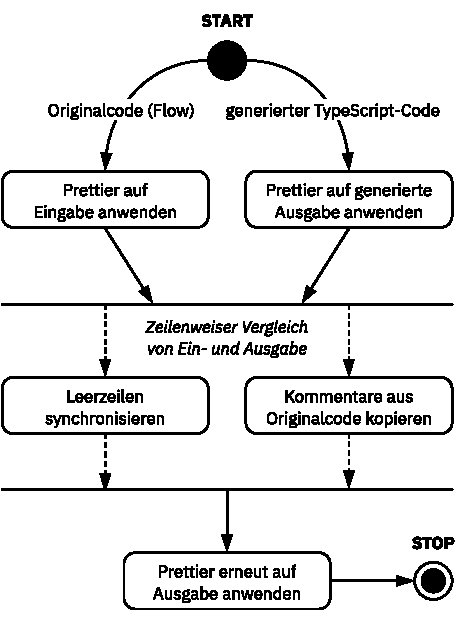
\includegraphics[width=.62\textwidth]{src/figures/formatting.pdf}
      \end{figure}
    \end{frame}

    \begin{frame}[noframenumbering]
      \frametitle{Nicht äquivalent übersetzbare Flow-Funktionen}
      \begin{itemize}
        \item \textit{Existential type}
        \item Beliebige Typen in Index-Signaturen von Objekttypen
        \item \textit{Opaque type}
        \item Expliziter Rückgabewert von Konstruktoren
        \item Varianz\footnote{TypeScript unterstützt nur Kovarianz}
      \end{itemize}
    \end{frame}

    \begin{frame}[noframenumbering]
      \frametitle{Vergleich mit Kikura~\autocite{KIKURA} und Barabash~\autocite{BARABASH}}
      \begin{itemize}
        \item während der Ausarbeit parallel entstandene Ansätze zur Transpilierung von Flow
        \item Test mit Fixture-Dateien
        \item Absturz in 54,8\% bzw. 9,7\% der Fälle
        \item fehlerhafte Transformtionen in 1,9\% bzw. 11,0\% der Fälle
        \item außerdem: zum Teil Abstürze bei bestimmter (valider) Eingabesyntax
      \end{itemize}
    \end{frame}

    \begin{frame}[noframenumbering]
      \frametitle{Unterstützung von Bibliotheken (Top 12) }
      {
        \footnotesize
        \begin{tabu} to \textwidth {@{}lrrr@{}}
          \midrule
          \rowfont[l]{} Bibliothek & Version & Verfügb. Flow & Verfügb. TypeScript \\
          \midrule
          react             & 16.11 &	16.11~~~~~~\code{\small I}  & 16.11~~~~~~\code{\small E} \\
          styled-components &   4.4 &	  4.x~~~~~~\code{\small E}  &   4.1~~~~~~\code{\small E} \\
          @storybook/react  &   5.2 &   5.x~~~~~~\code{\small E}  &   4.0~~~~~~\code{\small E} \\
          chai              &   4.2 &   4.x~~~~~~\code{\small E}  &   4.2~~~~~~\code{\small E} \\
          react-redux       &   7.1 &	  7.x~~~~~~\code{\small E}  &   7.1~~~~~~\code{\small E} \\
          react-apollo      &   3.1 &                        ---  &   3.1~~~~~~\code{\small I} \\
          react-router-dom  &   5.1 &   5.x~~~~~~\code{\small E}  &   5.1~~~~~~\code{\small E} \\
          react-loadable    &   5.5 &   5.x~~~~~~\code{\small E}  &   5.5~~~~~~\code{\small E} \\
          lodash            &  4.17 &   4.x~~~~~~\code{\small E}  &  4.14~~~~~~\code{\small E} \\
          react-router      &   5.1 &   5.x~~~~~~\code{\small E}  &   5.1~~~~~~\code{\small E} \\
          es6-error         &   4.1 &   4.x~~~~~~\code{\small E}  &   4.1~~~~~~\code{\small I} \\
          react-motion      &   0.5 &                        ---  &  0.29~~~~~~\code{\small E} \\
          \midrule
        \end{tabu}
      }
    \end{frame}

    \begin{frame}[noframenumbering]
      \frametitle{Testsysteme}
      {
        \footnotesize
        \textbf{System A}\\
          AMD Phenom II X6 1055T Prozessor mit 2,9~GHz\footnote{Jeweils Grundtakt des Prozessors} und 6~Rechenkernen (2010), 16~GB Arbeitsspeicher, Solid State Drive, Arch Linux\\[1em]
        \textbf{System B}\\
          Intel Core i5-4258U Prozessor mit 2,4~GHz und 4~Rechenkernen (2013), 8~GB Arbeitsspeicher, Solid State Drive, Arch Linux\\[1em]
        \textbf{System C}\\
          Intel Core i5-4210M Prozessor mit 2,6~GHz und 4~Rechenkernen (2014), 16~GB Arbeitsspeicher, Solid State Drive, Arch Linux\\[1em]
        \textbf{System D}\\
          Intel Core i7-6700 Prozessor mit 3,4~GHz und 8~Rechenkernen (2015), 32~GB Arbeitsspeicher, Solid State Drive, Debian Linux
      }
    \end{frame}

    \begin{frame}[noframenumbering,allowframebreaks]
      \frametitle{Performance -- Vollständige Typüberprüfung}
      {
        \footnotesize
        \textbf{Projekt Components}\\[1em]
        \begin{tabu} to \textwidth {@{}rrr|rr|r@{}}
          \midrule
          {} & \multicolumn{2}{l|}{Flow} & \multicolumn{2}{l|}{TypeScript} \\
          \rowfont[c]{} S & Laufzeit & s & Laufzeit & s & rel. $\Delta$  \\
          \midrule
          A & 7,87 & 0,09 & 15,50 & 0,08 & 97,0\% \\
          B & 6,86 & 0,05 & 10,59 & 0,06 & 54,4\% \\
          C & 6,50 & 0,02 &  9,56 & 0,05 & 47,1\% \\
          D & 3,38 & 0,02 &  6,41 & 0,04 & 89,6\% \\
          \midrule
        \end{tabu}
        \\[.75em]
        Laufzeit in Sekunden mit Standardabweichung s

        \framebreak

        \textbf{Projekt Helios}\\[1em]
        \begin{tabu} to \textwidth {@{}rrr|rr|r@{}}
          \midrule
          {} & \multicolumn{2}{l|}{Flow} & \multicolumn{2}{l|}{TypeScript} \\
          \rowfont[c]{} S & Laufzeit & s & Laufzeit & s & rel. $\Delta$  \\
          \midrule
          A & 12,20 & 0,16 & 13,06 & 0,70 &   7,1\% \\
          B & 10,90 & 0,33 &  8,49 & 0,16 & -22,1\% \\
          C & 11,70 & 0,07 &  7,63 & 0,04 & -34,8\% \\
          D &  5,15 & 0,02 &  4,94 & 0,03 &  -4,1\% \\
          \midrule
        \end{tabu}
        \\[.75em]
        Laufzeit in Sekunden mit Standardabweichung s
      }
    \end{frame}

    \begin{frame}[noframenumbering,allowframebreaks]
      \frametitle{Performance -- Einfluss Parallelisierung}
      {
        \footnotesize

        \textbf{Projekt Components}\\[1em]
        \begin{tabu} to \textwidth {@{}rrr|rr|r@{}}
          \midrule
          {} & \multicolumn{2}{l|}{Flow} & \multicolumn{2}{l}{TypeScript} \\
          \rowfont[c]{} K & Laufzeit & s & Laufzeit & s & rel. $\Delta$   \\
          \midrule
          1 & 10,59 & 0,03 & 10,13 & 0,03 & -4,3\% \\
          2 &  6,19 & 0,02 &  6,85 & 0,05 & 10,7\% \\
          3 &  4,74 & 0,03 &  6,50 & 0,02 & 37,1\% \\
          4 &  4,05 & 0,03 &  6,43 & 0,02 & 58,8\% \\
          5 &  3,79 & 0,04 &  6,48 & 0,02 & 71,0\% \\
          6 &  3,63 & 0,02 &  6,41 & 0,04 & 76,6\% \\
          7 &  3,52 & 0,02 &  6,40 & 0,03 & 81,8\% \\
          8 &  3,42 & 0,02 &  6,40 & 0,03 & 87,1\% \\
          \midrule
        \end{tabu}

        \framebreak

        \textbf{Projekt Helios}\\[1em]
        \begin{tabu} to \textwidth {@{}rrr|rr|r@{}}
          \midrule
          {} & \multicolumn{2}{l|}{Flow} & \multicolumn{2}{l}{TypeScript} \\
          \rowfont[c]{} K & Laufzeit & s & Laufzeit & s & rel. $\Delta$   \\
          \midrule
          1 & 17,26 & 0,05 & 8,81 & 0,01 & -49,0\% \\
          2 &  9,61 & 0,04 & 5,44 & 0,04 & -43,4\% \\
          3 &  7,23 & 0,03 & 5,03 & 0,02 & -30,4\% \\
          4 &  6,16 & 0,04 & 4,95 & 0,01 & -19,6\% \\
          5 &  5,82 & 0,03 & 5,04 & 0,15 & -13,4\% \\
          6 &  5,51 & 0,03 & 4,94 & 0,03 & -10,3\% \\
          7 &  5,31 & 0,03 & 4,93 & 0,03 &  -7,2\% \\
          8 &  5,16 & 0,02 & 4,94 & 0,03 &  -4,3\% \\
          \midrule
        \end{tabu}
      }
    \end{frame}

    \begin{frame}[plain,allowframebreaks,noframenumbering]
      \frametitle{Quellenverzeichnis}
      \printbibliography
    \end{frame}
\end{document}
